% Segmentator white paper. Build with `make pdf` (LuaLaTeX inside the TeX Live
% image); every number, table and catalogue row it \inputs comes out of
% generated/ and is written by bench.py, figures.py or catalogue.py.
\documentclass[11pt, a4paper, DIV=11, parskip=half-]{scrartcl}

\usepackage{fontspec}
\setmainfont{Libertinus Serif}
\setsansfont{Libertinus Sans}
\setmonofont{Libertinus Mono}[Scale=MatchLowercase]

\usepackage[english]{babel}
\usepackage{microtype}
\usepackage[a4paper, margin=28mm, bottom=32mm]{geometry}
\usepackage{graphicx}
\usepackage{booktabs}
\usepackage{longtable}
\usepackage{array}
\usepackage{caption}
\usepackage{subcaption}
\usepackage{listings}
\usepackage{xcolor}
\usepackage{pgfplots}
\usepackage{pgfplotstable}
\pgfplotsset{compat=1.18}

% The palette is the documentation diagrams' own, so a restyled SVG and the
% page it sits on are the same design rather than two.
\definecolor{ink}{HTML}{1F2933}
\definecolor{muted}{HTML}{52606D}
\definecolor{rule}{HTML}{CBD2D9}
\definecolor{accent}{HTML}{1F6FEB}
\definecolor{amber}{HTML}{B44D12}
\definecolor{green}{HTML}{1F8A70}
\definecolor{violet}{HTML}{5B21B6}

\usepackage[colorlinks=true, allcolors=accent]{hyperref}

\addtokomafont{disposition}{\sffamily\color{ink}}
\addtokomafont{caption}{\small\color{muted}}
\addtokomafont{captionlabel}{\bfseries\color{ink}}
\setcapindent{0pt}

\usepackage[backend=biber, style=numeric, sorting=none, maxbibnames=8]{biblatex}
\addbibresource{bib/refs.bib}

% --- code and diff listings ------------------------------------------------ %
\lstdefinestyle{yaml}{
  basicstyle=\ttfamily\footnotesize\color{ink},
  commentstyle=\color{muted}\itshape,
  keywordstyle=\color{violet},
  columns=fullflexible, breaklines=true, frame=none, showstringspaces=false,
  morecomment=[l]{\#},
}
\lstdefinelanguage{diff}{
  % [f] anchors each marker to column 0. A line-scoped delimiter would match the
  % `-` that starts every YAML list item and paint the context lines red.
  morecomment=[f][\color{green}]{+},
  morecomment=[f][\color{amber}]{-},
  morecomment=[f][\color{accent}]{@@},
  morecomment=[f][\color{muted}\itshape]{diff\ },
}
\lstdefinestyle{diff}{
  language=diff,
  basicstyle=\ttfamily\scriptsize\color{ink},
  columns=fullflexible, breaklines=false, frame=none, showstringspaces=false,
  aboveskip=2pt, belowskip=2pt,
}
\lstset{style=yaml}

% Table rows come from generated/ via the TeX primitive, not LaTeX's \input:
% LaTeX's wraps the file in a way that leaves a token between the last \\ and
% the following \bottomrule, and booktabs' \noalign then lands mid-row.
\makeatletter
\newcommand{\inputrows}[1]{\@@input #1 }
\makeatother

% --- generated inputs: numbers the prose quotes ---------------------------- %
\newcommand{\BenchBaselineFps}{1063}
\newcommand{\BenchMotionFps}{81}
\newcommand{\BenchMotionFpsVGA}{21}
\newcommand{\BenchMotionFpsHD}{6}
\newcommand{\BenchSlowestVideo}{motion}
\newcommand{\BenchSlowestVideoFps}{81}
\newcommand{\BenchTextureMs}{90}
\newcommand{\BenchDearestStage}{farneback}
\newcommand{\BenchDearestMs}{11.0}
\newcommand{\BenchDearestShare}{93}
\newcommand{\BenchCostConfig}{motion}

\newcommand{\NumStages}{43}
\newcommand{\NumSources}{3}
\newcommand{\NumSinks}{6}
\newcommand{\NumFamilies}{7}
\newcommand{\FamilyList}{\texttt{color}, \texttt{keypoints}, \texttt{mask}, \texttt{motion}, \texttt{preprocess}, \texttt{structure}, \texttt{texture}}

\newcommand{\OptStages}{13}
\newcommand{\OptFindings}{7}
\newcommand{\OptProved}{4}
\newcommand{\OptSampled}{3}
\newcommand{\OptKept}{4}
\newcommand{\OptFrames}{16}
\newcommand{\OptKeptList}{\texttt{static\_mask}, \texttt{apply\_mask}, \texttt{gray}, \texttt{contours}}

\newcommand{\LegacyLOC}{217}
\newcommand{\LegacyModules}{6}
\newcommand{\LegacyFiles}{3}
\newcommand{\LegacyInsertions}{10}
\newcommand{\LegacyDeletions}{33}
\newcommand{\LegacyChanged}{43}


% The field-footage confirmation is the one measurement that needs media not in
% this repository. Without it the sentence that quotes it is left out entirely,
% rather than the document carrying a number nobody can reproduce.
\newif\iffieldnumbers
\IfFileExists{generated/field-numbers.tex}{\newcommand{\FieldSlowest}{motion}
\newcommand{\FieldSlowestFps}{87}
\newcommand{\FieldFrames}{900}
\newcommand{\FieldSynthetic}{81}
\fieldnumberstrue}{}

\title{Segmentator: Configuration-Driven Segmentation Pipelines for Industrial Video}
\subtitle{Composing \NumStages{} classical operators without writing code}
\author{Mateus G. Machado}
\date{August 2026}

\begin{document}

% --------------------------------------------------------------------------- %
% Title page
% --------------------------------------------------------------------------- %
\begin{titlepage}
\sffamily
\noindent{\color{accent}\rule{\textwidth}{2.5pt}}\par
\vspace{2cm}

\noindent{\Huge\bfseries\color{ink} Segmentator}\par
\vspace{6mm}
\noindent{\LARGE\color{ink} Configuration-Driven Segmentation\\Pipelines for Industrial Video}\par
\vspace{5mm}
\noindent{\large\color{muted} Composing \NumStages{} classical operators without writing code}\par

\vspace{2.4cm}
\noindent{\large\color{ink} Mateus G. Machado}\par
\vspace{2mm}
\noindent{\color{muted} SENAI Institute for Innovation in Information\\
and Communication Technologies (ISI-TICs)\\
Recife, Brazil}\par

\vfill
\noindent{\color{rule}\rule{\textwidth}{0.6pt}}\par
\vspace{3mm}
\noindent\begin{minipage}[t]{0.48\textwidth}
  \small\color{muted}
  Version 0.5.1 \quad August 2026\\
  Software: \href{https://github.com/goncamateus/segmentator}{github.com/goncamateus/segmentator}\\
  released under the MIT licence
\end{minipage}\hfill
\begin{minipage}[t]{0.48\textwidth}
  \small\color{muted}
  This document is licensed \href{https://creativecommons.org/licenses/by/4.0/}{CC BY 4.0}.\\
  Code excerpts remain under the MIT licence.
\end{minipage}
\end{titlepage}

% --------------------------------------------------------------------------- %
% Sections only: the subsection level spills the contents onto a second page
% and earns nothing in a document this size.
\setcounter{tocdepth}{1}
\tableofcontents
\clearpage

\begin{abstract}
\noindent
Segmenting a gas plume from low-resolution thermal video admits no single correct
method: the plume has no stable edge, shape or colour, and which combination of
classical operators works is an empirical question about the footage. The
predecessor to this work answered it with a hardcoded script, which fused the
recipe with the machinery and made every further question a code edit. This paper
describes Segmentator, an engine in which the recipe is a declarative
\texttt{source $\rightarrow$ stages $\rightarrow$ sinks} configuration over
\NumStages{} registered operators, composed by ordering alone with no runtime
branching, authored in a visual editor generated from the same registry the
batch runner builds from. The engine additionally audits its own chains,
separating findings it can prove from findings it can only fail to falsify. On
one CPU core with no GPU, every video recipe exceeds the 15~fps field frame rate
at $320\times240$, the slowest at \BenchSlowestVideoFps~fps. No labelled ground
truth exists for this footage, so no detection accuracy is claimed.

\vspace{2mm}
\noindent\textbf{Keywords:} video segmentation; configuration-driven pipelines;
classical computer vision; thermal imaging; gas plume detection; reproducibility.
\end{abstract}

\section{Executive summary}

Segmentator is an engine for image and video segmentation in which the method is
a configuration file rather than a program. It began as one hardcoded script for
pulling a gas plume out of thermal video; generalising that script into a
declarative \texttt{source $\rightarrow$ stages $\rightarrow$ sinks} format is
the whole of the project. An operator composes a recipe from \NumStages{}
classical operators, tunes it against live footage in a visual editor, and the
same file then runs unattended over a batch. Changing the method --- a different
background model, a different detector, a different order --- is an edit to that
file, reviewed and re-run in seconds, rather than an edit to the code that also
owns frame decoding and video encoding.

What this document reports is a working engine, measured. It runs faster than
real time at field resolution on a single CPU core, its component catalogue and
every number printed here are generated from the code itself, and all of it
reproduces from the repository with one command. What it does not report is
detection accuracy: no labelled ground truth exists for this footage, so this
paper contains no detection rate, no false-alarm rate and no comparison against a
learned model. §\ref{sec:limitations} states that boundary and the rest of them
plainly.

\begin{itemize}
  \item A segmentation recipe is a YAML file: changing the method is a config
        edit, not a code edit.
  \item \NumStages{} operators across \NumFamilies{} families compose by ordering
        alone --- no runtime branching, no feature flags.
  \item An operator tunes the chain visually with a live per-stage preview, and
        the same file then runs headless in batch.
  \item The tool audits its own chains: it proves what can be proved, samples the
        rest, and says out loud which is which.
  \item Real time at field resolution on one CPU core and no GPU: every video
        recipe clears 15~fps at $320\times240$, the slowest
        (\texttt{\BenchSlowestVideo}) at \BenchSlowestVideoFps~fps.
\end{itemize}

\section{The problem}
% INTENT: gas plume segmentation from low-resolution thermal video. Why the
% first working answer was a hardcoded script, why that script was a dead end
% (every question about the footage meant editing Python), and why the problem
% generalises past gas: the recipe changes far more often than the machinery.

\section{Approach: the config is the program}
% INTENT: source -> stages -> sinks, and the claim that the ordered list *is*
% the composition. Registry as single source of truth for schema, editor
% palette and error messages simultaneously.

\begin{figure}[t]
  \centering
  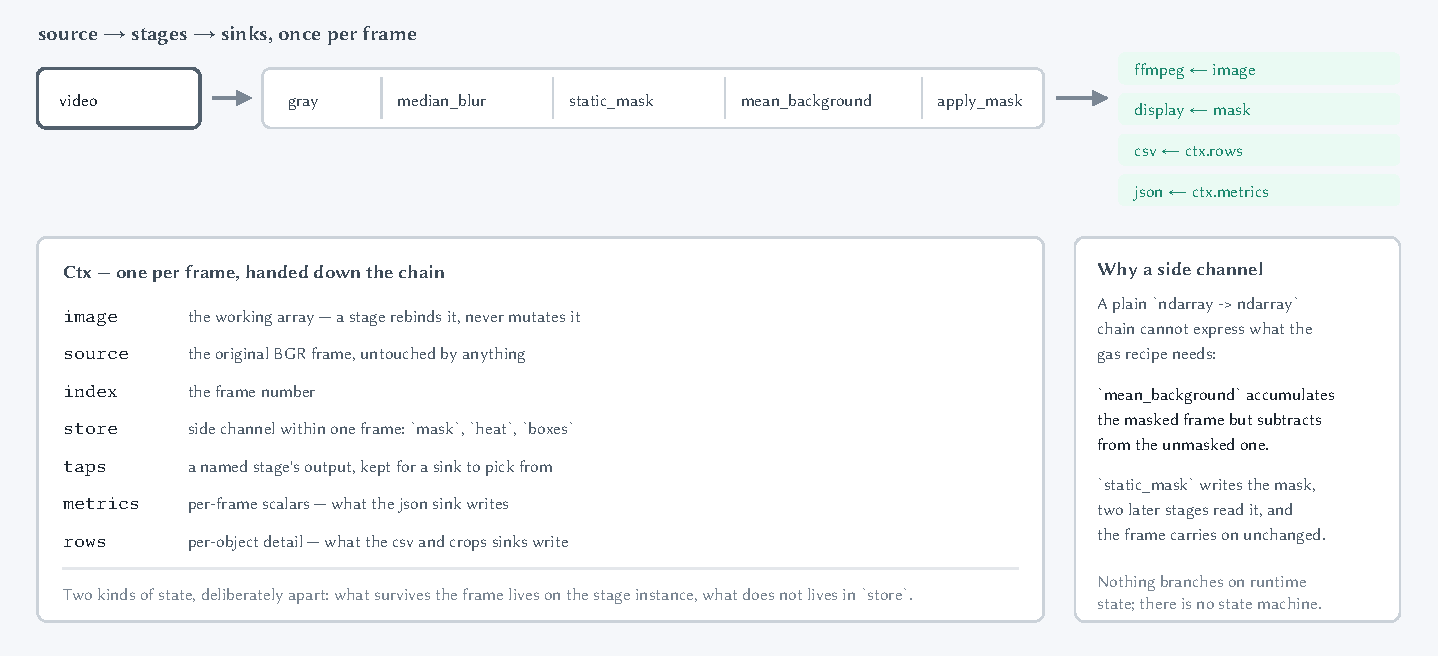
\includegraphics[width=\textwidth]{figures/pipeline-anatomy.pdf}
  \caption{A pipeline: one source, an ordered list of stages, one or more
    sinks, and the per-frame \texttt{Ctx} that carries state between them.}
  \label{fig:anatomy}
\end{figure}

% INTENT: a short YAML listing here, the baseline recipe, annotated.

\section{Architecture}
\label{sec:architecture}

\subsection{One object per frame}

Everything a stage can read or write for the frame in front of it lives on a
single object, \texttt{Ctx}, which the runner creates per frame and discards at
the end of it. It carries the working image, the untouched source frame, the
frame index, and four output channels that are kept apart on purpose:

\begin{description}
  \item[\texttt{store}] a side channel within one frame: an artifact one stage
    produces and a later stage consumes, such as the binary mask
    \texttt{static\_mask} publishes and \texttt{apply\_mask} reads. It is thrown
    away when the frame ends. State that has to survive between frames belongs on
    the stage instance instead, and the distinction is enforced by the fact that
    nothing carries \texttt{store} forward.
  \item[\texttt{taps}] a snapshot of the working image taken after each
    \emph{named} stage, so a sink can write a mid-chain frame instead of only the
    final one. Taps are filled by the runner, never by a stage. Keeping them out
    of \texttt{store} is what stops a stage named \texttt{mask} from shadowing the
    unrelated \texttt{store["mask"]} artifact --- a collision that would be
    invisible until it produced a wrong picture.
  \item[\texttt{metrics}] the per-frame scalars a stage measured:
    \texttt{edge\_px}, \texttt{contours}, \texttt{motion\_speed},
    \texttt{lbp\_entropy}. One dictionary per frame, and what the JSON sink
    writes.
  \item[\texttt{rows}] per-object detail --- one list of flat records per kind.
    This is separate from \texttt{metrics} because a single frame's
    \texttt{contours = 400} metric can have four hundred records behind it, and
    the CSV and crop sinks want those records, not the count.
\end{description}

A stage's contract is one method, \texttt{apply(ctx)}, and one rule: rebind
\texttt{ctx.image} to a new array, never modify the array in place. The rule
exists because \texttt{image} and \texttt{source} alias the same buffer when a
frame enters the chain and no defensive copy is taken --- at these frame rates a
per-frame copy is pure waste. A sink's contract is \texttt{write(ctx)}, returning
\texttt{False} to stop the run, which is how a preview window's quit key ends a
batch.

\subsection{Almost nothing has state}

Of the \NumStages{} stages, the ones that remember anything between frames are
the motion models and the background models, and they remember it on themselves.
There is exactly one state machine in the codebase --- the fixed background model
is either still accumulating its first $N$ frames or has fitted its mean and is
subtracting it --- and everything else is either a pure function of the current
frame or a running accumulation. That is a small fact with a large consequence:
it is why the analysis in §\ref{sec:optimizer} can rearrange a chain and know
what it is allowed to conclude, and why a chain's behaviour is a property of the
config rather than of the order somebody happened to click things.

\begin{figure}[t]
  \centering
  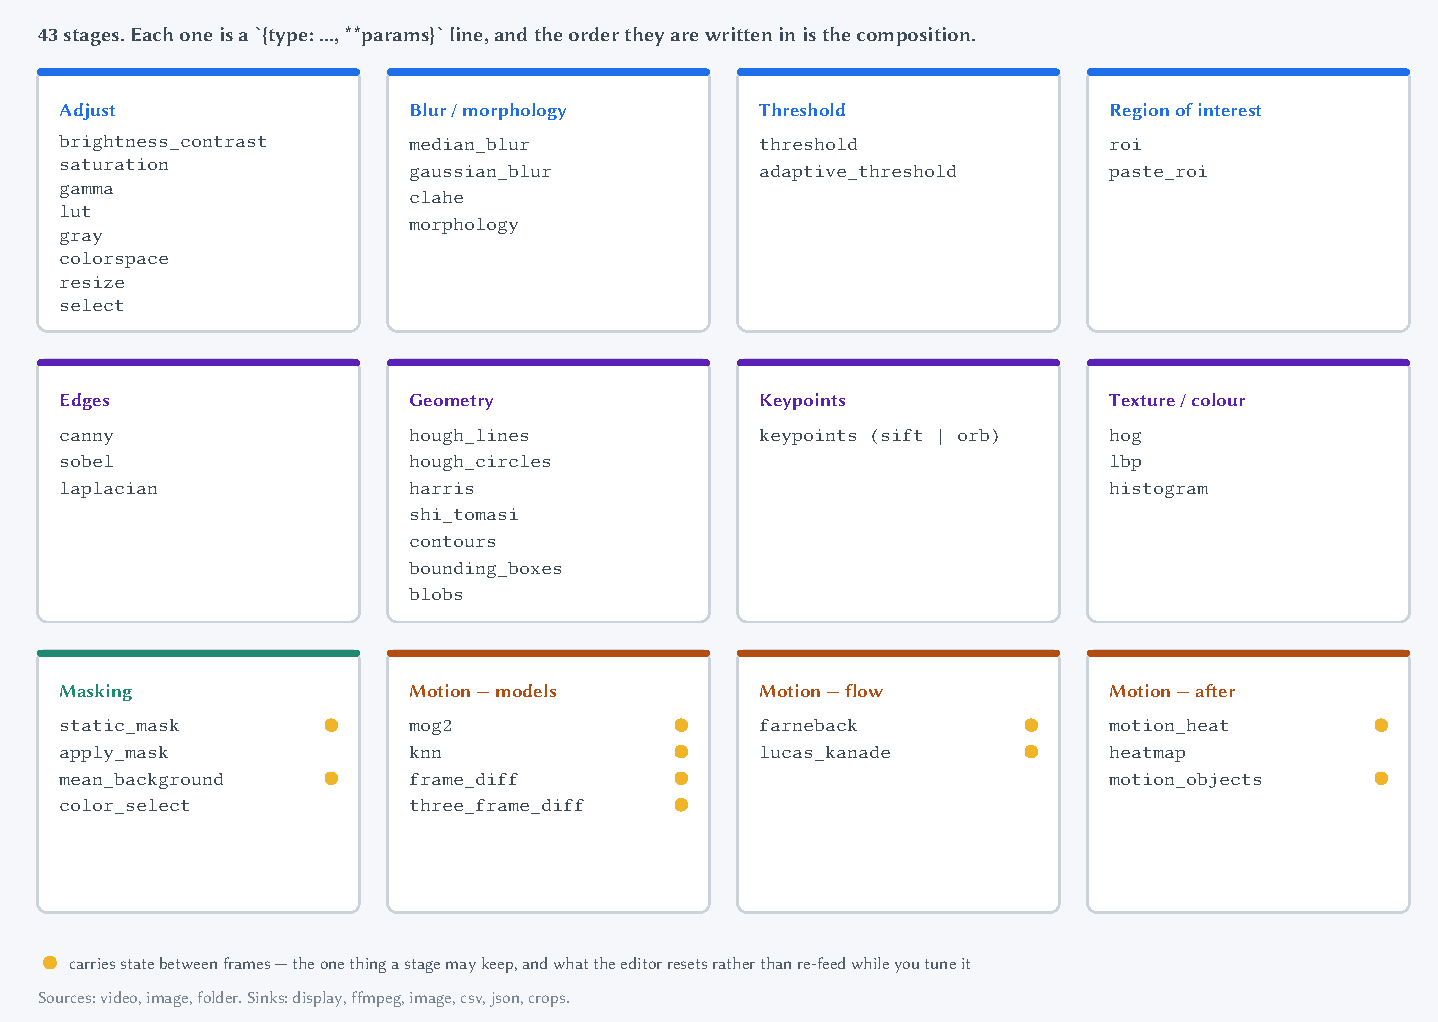
\includegraphics[width=\textwidth]{figures/stage-families.pdf}
  \caption{The \NumStages{} registered stages, grouped as the editor's palette
    groups them for browsing. The source tree divides them differently, into the
    \NumFamilies{} modules the appendix is organised by: \FamilyList{}.}
  \label{fig:families}
\end{figure}

\subsection{Where the operators come from}

None of the \NumStages{} operators is novel, and that is the point: each one is a
published method with three decades of use behind it, wrapped so that a config
can name it. The structure family implements Canny's edge detector
\cite{canny1986}, the Harris--Stephens corner response \cite{harris1988} and the
Shi--Tomasi selection criterion derived from it \cite{shi1994}, border-following
contour extraction \cite{suzuki1985}, and the progressive probabilistic Hough
transform for line segments \cite{matas2000}. The motion family covers sparse
Lucas--Kanade flow \cite{lucas1981}, dense flow by polynomial expansion
\cite{farneback2003}, and the two adaptive background subtractors --- the
improved Gaussian mixture model \cite{zivkovic2004} and its per-pixel density
estimation successor \cite{zivkovic2006}. The texture family provides histograms
of oriented gradients \cite{dalal2005} and multiresolution local binary patterns
\cite{ojala2002}; contrast-limited adaptive histogram equalisation
\cite{zuiderveld1994} sits in preprocessing. The implementations are OpenCV's
\cite{bradski2000} and scikit-image's \cite{vanderwalt2014} over NumPy arrays
\cite{harris2020numpy}; what this project contributes is the composition, not the
operators.

The two exceptions are worth naming because they are the only stages with no
published counterpart: the fixed region mask and the mean-of-$N$ background were
written for this project's own footage, and they are the two the predecessor
script already had.

\subsection{Why ordering has to be the composition}

\begin{figure}[t]
  \centering
  \begin{subfigure}[t]{0.48\textwidth}
    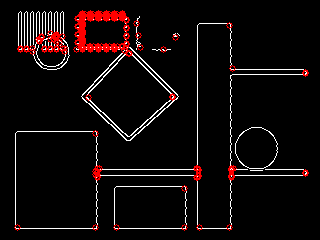
\includegraphics[width=\textwidth]{figures/ordering-edges-first.png}
    \caption{\texttt{canny} then \texttt{harris}: corners drawn onto the edge map.}
  \end{subfigure}\hfill
  \begin{subfigure}[t]{0.48\textwidth}
    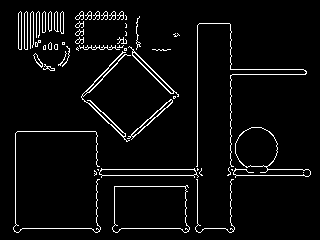
\includegraphics[width=\textwidth]{figures/ordering-corners-first.png}
    \caption{\texttt{harris} then \texttt{canny}: the corner markers are reduced
      to outlines, and an extra \texttt{gray} is needed to get there.}
  \end{subfigure}
  \caption{Ordering is the composition. The same two operators in opposite order
    are not two settings of one pipeline; they are two different pipelines.}
  \label{fig:ordering}
\end{figure}

Figure~\ref{fig:ordering} is the argument in one picture. Both panels run
\texttt{canny} and \texttt{harris} on the same frame with the same parameters.
On the left, edges are found first and the corner detector draws onto the edge
map, which is how you check that a corner detector is looking at the structure
you think it is. On the right, corners are drawn first and the edge detector then
runs over the markers and reduces them to outlines --- and because the marker
overlay is in colour, the reversed order also needs a \texttt{gray} stage
inserted to get there at all.

No flag distinguishes those two pipelines. A system that tried to express this
with options would need a \texttt{draw\_over\_edges} boolean, and then another
one for the next pair, and each would be a branch taken at runtime that somebody
has to read the source to understand. Making position the only composition
operator means the file shows what happens in the order it happens, and the cost
is paid in exactly one place: an operator that needs an image other than the one
in front of it has to say so. Several do --- \texttt{draw\_on: source} paints on
the original frame, \texttt{input: edges} reaches back to a named tap,
\texttt{mask: mask} reads a published artifact --- and those parameters are
visible in the config rather than implied by it.

\section{The editor}
% INTENT: the palette and every parameter form are generated from the same
% registry the CLI builds from, so nothing about a stage is declared twice.
% Live preview, mid-chain taps, transport.

\begin{figure}[t]
  \centering
  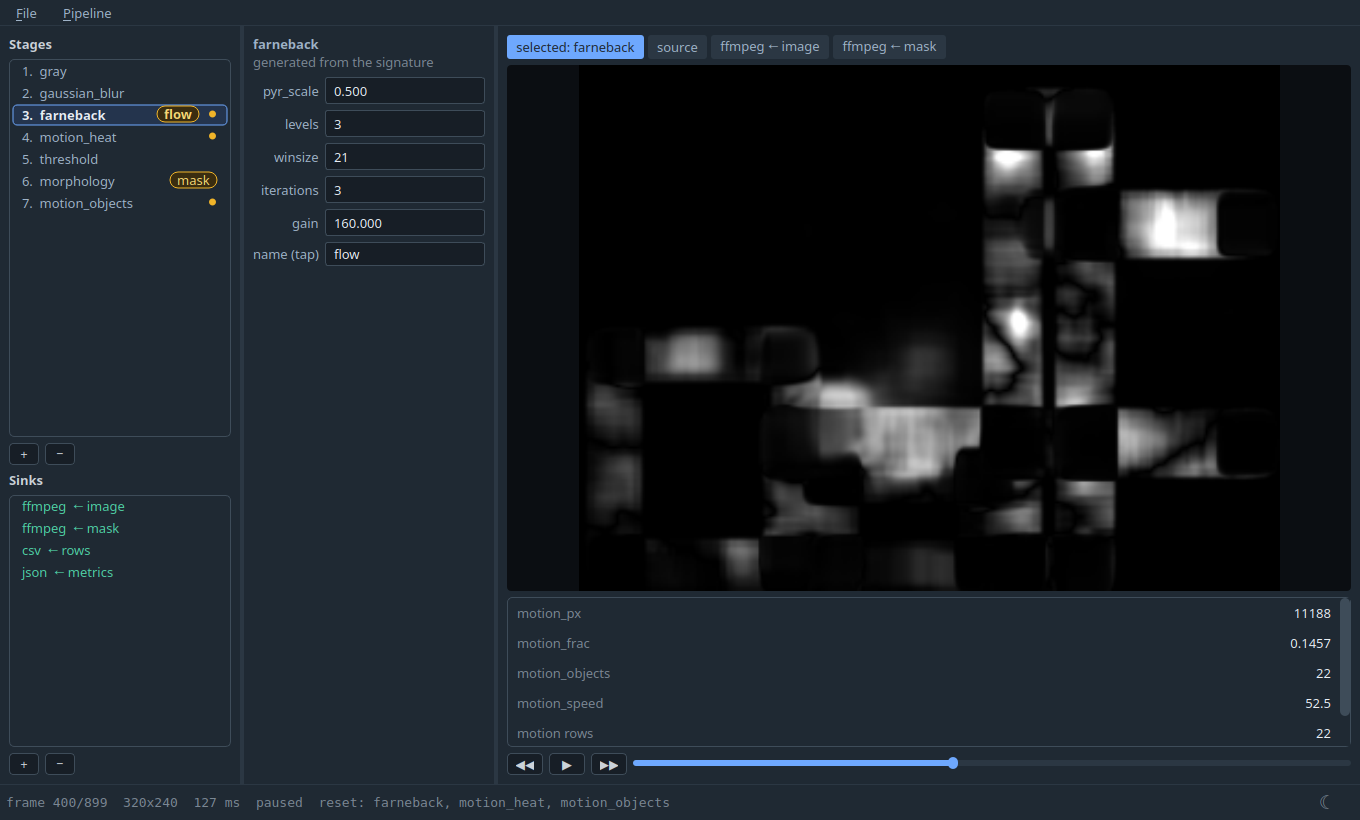
\includegraphics[width=\textwidth]{figures/editor-window.png}
  \caption{The editor on the \texttt{motion} recipe: stage list, the parameter
    form generated from \texttt{farneback}'s constructor signature, the live
    preview at frame 400, and the per-frame metrics beneath it.}
  \label{fig:editor}
\end{figure}

\section{Auditing a chain: proof, and the refusal to claim it}
% INTENT: the ratchet problem (stages accrete, nothing is taken back out).
% Structural findings are sound by construction; sampled findings are
% falsification only. SAMPLE_FLOOR, and why the tool proposes rather than
% applies. The `drop mean_background` row is the argument: no counterexample in
% \OptFrames{} frames is not the same as safe to remove.

\begin{table}[t]
  \centering
  \small
  \caption{Every finding the optimizer returns for a deliberately ratcheted
    \OptStages{}-stage chain: \OptProved{} proved and \OptSampled{} sampled.
    It leaves \OptKept{} stages alone (\OptKeptList{}).}
  \label{tab:findings}
  \begin{tabular}{@{}l p{0.30\textwidth} l p{0.26\textwidth} r@{}}
    \toprule
    Position & Proposal & Basis & Argument & Saved (ms) \\
    \midrule
    \inputrows{generated/optimize-findings.tex}
    \bottomrule
  \end{tabular}
\end{table}

\section{Validation}
% INTENT: three legs. (1) the suite: 301 tests, every example config driven end
% to end as a registry-drift guard, the editor covered headless. (2) synthetic
% media: what it is, what it deliberately is not (no physical gas model), and
% why publishing it matters more than a field frame would. (3) the measurements
% below, every one of which regenerates with `make bench`.

\begin{figure}[t]
  \centering
  \begin{subfigure}[t]{0.32\textwidth}
    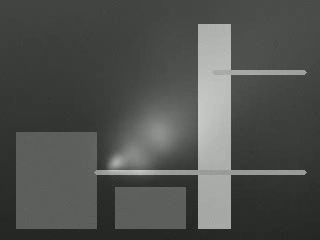
\includegraphics[width=\textwidth]{figures/plume-source.png}
    \caption{source frame}
  \end{subfigure}\hfill
  \begin{subfigure}[t]{0.32\textwidth}
    
\includegraphics[width=\textwidth]{figures/plume-roi.png}
    \caption{\texttt{static\_mask}: the region of interest}
  \end{subfigure}\hfill
  \begin{subfigure}[t]{0.32\textwidth}
    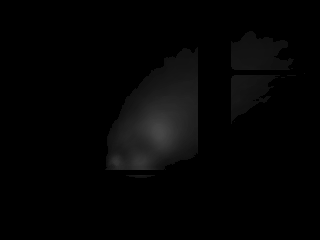
\includegraphics[width=\textwidth]{figures/plume-subtracted.png}
    \caption{after \texttt{mean\_background}}
  \end{subfigure}

  \vspace{3mm}
  \begin{subfigure}[t]{0.32\textwidth}
    
\includegraphics[width=\textwidth]{figures/plume-motion-mask.png}
    \caption{\texttt{farneback} thresholded}
  \end{subfigure}\hfill
  \begin{subfigure}[t]{0.32\textwidth}
    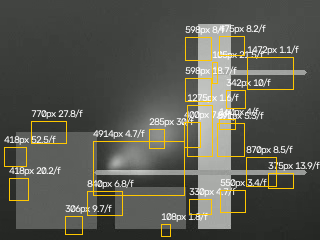
\includegraphics[width=\textwidth]{figures/plume-objects.png}
    \caption{\texttt{motion\_objects}, untuned for this scene}
  \end{subfigure}\hfill
  \caption{The \texttt{baseline} and \texttt{motion} recipes on the synthetic
    plume clip, frame 400. Every panel is a tap out of a real run.}
  \label{fig:plume}
\end{figure}

\begin{figure}[t]
  \centering
  \begin{subfigure}[t]{0.24\textwidth}
    
\includegraphics[width=\textwidth]{figures/geom-edges.png}
    \caption{\texttt{canny}}
  \end{subfigure}\hfill
  \begin{subfigure}[t]{0.24\textwidth}
    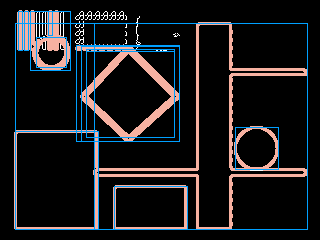
\includegraphics[width=\textwidth]{figures/geom-contours.png}
    \caption{\texttt{contours}}
  \end{subfigure}\hfill
  \begin{subfigure}[t]{0.24\textwidth}
    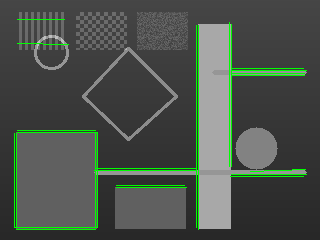
\includegraphics[width=\textwidth]{figures/geom-lines.png}
    \caption{\texttt{hough\_lines}}
  \end{subfigure}

  \vspace{3mm}
  \begin{subfigure}[t]{0.24\textwidth}
    
\includegraphics[width=\textwidth]{figures/geom-hog.png}
    \caption{\texttt{hog}}
  \end{subfigure}\hfill
  \begin{subfigure}[t]{0.24\textwidth}
    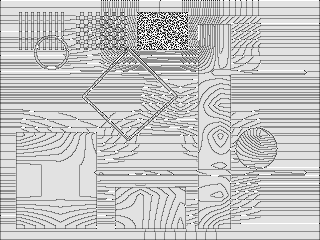
\includegraphics[width=\textwidth]{figures/geom-lbp.png}
    \caption{\texttt{lbp}}
  \end{subfigure}
  \caption{The structure and texture families on the synthetic geometry still.
    A drifting plume gives these operators nothing to describe, which is why
    the scene exists.}
  \label{fig:geometry}
\end{figure}

\begin{table}[t]
  \centering
  \small
  \caption{End-to-end throughput, sinks included, median of three runs on one
    core of an AMD Ryzen 5 5600X. No GPU is used.}
  \label{tab:throughput}
  \begin{tabular}{@{}llrrr@{}}
    \toprule
    Recipe & Resolution & Frames & ms/frame & fps \\
    \midrule
    \inputrows{generated/bench-throughput.tex}
    \bottomrule
  \end{tabular}
\end{table}

\begin{table}[t]
  \centering
  \small
  \caption{Where one frame's budget goes in the \texttt{\BenchCostConfig{}}
    recipe at $320\times240$, sinks excluded.}
  \label{tab:stagecost}
  \begin{tabular}{@{}lrr@{}}
    \toprule
    Stage & ms & \% of frame \\
    \midrule
    \inputrows{generated/bench-stagecost.tex}
    \bottomrule
  \end{tabular}
\end{table}

\begin{figure}[t]
  \centering
  \begin{tikzpicture}
    \begin{axis}[
      width=0.68\textwidth, height=6.2cm,
      xlabel={pixels per frame}, ylabel={frames per second},
      xmode=log, ymode=log, log basis x=10, log basis y=10,
      grid=both, major grid style={rule}, minor grid style={rule!40},
      xmin=6e4, xmax=1.1e6,
      legend style={draw=rule, font=\small, at={(1.03,1)}, anchor=north west},
      tick label style={color=muted}, label style={color=ink},
      cycle list={{accent}, {green}, {amber}, {violet}, {muted}, {ink}},
    ]
      \foreach \column/\label in {baseline/baseline, gasvid/gasvid1,
                                  mog/mog2\_contours, motion/motion,
                                  structure/structure, texture/texture} {
        \addplot+[mark=*, thick] table[x=pixels, y=\column] {generated/bench-sweep.dat};
        \addlegendentryexpanded{\texttt{\label}}
      }
      % 15 fps: the frame rate of the field footage this project started from.
      \addplot[dashed, amber, thick, forget plot, domain=6e4:1.1e6] {15};
    \end{axis}
  \end{tikzpicture}
  \caption{Throughput against frame size, both axes logarithmic. The dashed
    line is 15~fps, the frame rate of the field footage this project started
    from: every video recipe clears it at $320\times240$, and the motion chain
    stops clearing it before $1280\times720$. \texttt{structure} and
    \texttt{texture} describe a single still, so their figure is images per
    second, not a rate they have to keep up with.}
  \label{fig:sweep}
\end{figure}

\section{What this replaced, and what it does not replace}
% INTENT: two comparisons. (1) the predecessor: 217 LOC over six files, one
% hardcoded recipe, measured. (2) deep learning: cost of entry (no labels
% exist), complementary (this tool is how labels get made), interpretability --
% and the concession that a trained model with labels and a GPU would very
% likely win on accuracy.

\begin{figure}[t]
  \begin{subfigure}[t]{\textwidth}
    \lstinputlisting[style=diff]{generated/legacy-mog2.diff}
    \caption{The predecessor architecture: \LegacyChanged{} changed lines
      across \LegacyFiles{} files, one module deleted outright.
      \emph{Reconstructed} --- the predecessor never supported MOG2, so this is
      the equivalent change, not a recovered commit; both trees are in
      \texttt{docs/whitepaper/legacy/}.}
  \end{subfigure}

  \vspace{4mm}
  \begin{subfigure}[t]{\textwidth}
    \lstinputlisting[style=diff]{generated/config-mog2.diff}
    \caption{The same change here: one line.}
  \end{subfigure}
  \caption{Swapping a fixed mean background for adaptive MOG2.}
  \label{fig:diff}
\end{figure}

\section{Limitations and maturity}
\label{sec:limitations}

The honest summary of where this stands is: validated, not deployed. Concretely.

\paragraph{There is no accuracy claim in this document, anywhere.} No labelled
ground truth exists for the footage, so there is no intersection-over-union, no
precision or recall, no false-alarm rate and no detection-limit figure. Every
number in §\ref{sec:validation} is a throughput or a cost. A reader should treat
the absence as deliberate: the pipeline visibly separates a plume from a
background, and how well it does so against a human's judgement is unmeasured.

\paragraph{One camera, one scene type.} Everything here was developed against a
fixed thermal camera looking at one installation, and validated on synthetic
media built to resemble it. Generalisation to a different sensor, a different
spectral band, a moving camera or a cluttered outdoor scene is untested, and
several of the design choices --- a fixed region mask, a mean-of-$N$ background
--- assume a static camera and would need replacing rather than retuning.

\paragraph{A recipe is tuned to a scene, and does not travel.}
Figure~\ref{fig:plume}(e) is the demonstration: the shipped \texttt{motion}
recipe, run unmodified on a scene it was not tuned for, reports twenty-two
objects where a reader sees one plume. Nothing is broken --- the parameters are
simply wrong for that footage. This is the actual operating cost of the approach,
and the editor exists because of it: the tool makes retuning cheap, it does not
make it unnecessary.

\paragraph{Single-threaded, CPU only.} One core, one frame at a time. There is a
GPU in the benchmark machine and the engine never touches it. Frames are
processed in a single forward pass with no parallelism across frames, stages or
sinks, and no attempt has been made at any of the three.

\paragraph{Batch, not online.} The engine reads a file and writes files. There is
no streaming input from a live camera, no alerting, no persistence beyond CSV and
JSON on disk, and no operator-facing runtime --- the editor is a tuning tool, not
a control room display. Nothing in the architecture forbids these; none of them
is written.

\paragraph{No physical calibration.} A plume's segmented area is measured in
pixels, and its motion in pixels per frame. Converting either into a
concentration, a flow rate or a leak volume needs sensor calibration, scene
geometry and a physical model, none of which is in scope here.

\paragraph{Maturity.} By the TRL scale this is a level~4 result: the components
are validated together in a representative setting, on real footage, with a
reproducible measurement of what they cost. It is not hardened for on-site
deployment, has not run unattended, and has no failure-handling story beyond
raising an exception and stopping.

\section{Next phase}
% INTENT: five items, each tied to a limitation above. Labelled evaluation set
% and quantitative validation; multi-scene generalisation; parallel and
% streaming execution; hardening for on-site deployment; using the classical
% output as bootstrap labels for a learned model.


\printbibliography[heading=bibnumbered]

\appendix
\section{Component catalogue}
\label{sec:catalogue}

Table~\ref{tab:catalogue} is generated by \texttt{docs/whitepaper/catalogue.py}
directly from the component registry: names come from the \texttt{@register}
decorators, and the grouping from the module each class lives in. It is
regenerated as a prerequisite of building this PDF, so it cannot list a component
that does not exist or omit one that does --- which is the same guarantee, from
the same table, that the config schema and the editor's palette get
(§\ref{sec:architecture}).

Each component's parameters, defaults and one-line purpose are in the published
documentation at \url{https://goncamateus.github.io/segmentator/}, in English and
Portuguese, and in the repository under \texttt{docs/en/stages.md}. The same
generator emits that longer form; it is left out here because a reader who needs
a parameter's default needs it next to a config they are editing, not in a PDF.

\begin{table}[h]
  \small
  \caption{The \NumStages{} stages by module family, and the \NumSources{}
    sources and \NumSinks{} sinks.}
  \label{tab:catalogue}
  \begin{tabular}{@{}l p{0.78\textwidth}@{}}
    \toprule
    Family & Components \\
    \midrule
    \inputrows{generated/catalogue-compact.tex}
    \bottomrule
  \end{tabular}
\end{table}


\end{document}
